\documentclass[11pt,twoside,a4paper]{report}

\usepackage{graphicx}
% Use Palatino font family
\usepackage{palatino}
\usepackage{amsmath}
\usepackage{amssymb}
\usepackage{breqn}

\usepackage{afterpage}
% ----------------------
% Page layout details
% ----------------------
\usepackage[top=2cm,bottom=2cm,inner=2cm,outer=3cm,bindingoffset=1cm,
            includehead,includefoot,twoside]{geometry}

% Change the default look of section headings
\usepackage[bf,sf,compact]{titlesec}

\titleformat{\part}[display]
{\bfseries\sffamily\Huge}
{\filcenter\bfseries\sffamily\LARGE Part \thepart}
{1ex}
{\vspace{1ex}%
\filcenter}

\titleformat{\chapter}[display]
{\bfseries\sffamily\LARGE}
{\filleft\bfseries\sffamily\Huge\thechapter}
{1ex}
{\vspace{1ex}%
\filleft}

\titleformat{\section}
{\bfseries\sffamily\large}
{\thesection}
{1ex}
{\vspace{0.5ex}}

\titlespacing{\section}{0pt}{2.0ex}{0.5ex}


%%%%%%%%%%%%%%%%%%%%%%%%%%%%%%%%%%%%%%%%%%%%%%%%%%%%%%
% Table of Contents formatting
%%%%%%%%%%%%%%%%%%%%%%%%%%%%%%%%%%%%%%%%%%%%%%%%%%%%%%
\usepackage{titletoc}
\contentsmargin{2.55em}

\titlecontents{part}
[0.0em] % 
{\addvspace{0.5em}}
{\bfseries\sffamily\large\contentslabel{0.0em}}
{\bfseries\sffamily\large\hspace*{-1.8em}}
{\hspace{1.0em}\bfseries\sffamily\large{}\contentspage}
[\addvspace{0.5em}]

\titlecontents{chapter}
[0.0em] % 
{\addvspace{0.5em}}
{\bfseries\sffamily\contentslabel{2.0em}}
{\bfseries\sffamily\hspace*{-2.0em}}
%{\titlerule*[1pc]{ }\bfseries\sffamily\contentspage}
{\hspace{1.0em}\bfseries\sffamily{}\contentspage}
[\addvspace{0.5em}]

\titlecontents{section}
[2.5em] % 
{}
{\sffamily\contentslabel{2.5em}}
{\sffamily\hspace*{0.0em}}
{\hspace{1.0em}\sffamily{}\contentspage}

\titlecontents{subsection}
[5.4em]
{}
{\sffamily\contentslabel{3.0em}}
{\sffamily\hspace*{0.0em}}
{\hspace{0.5em}\sffamily{}\contentspage}


% For better control of captions
\usepackage[font=small,labelfont=bf,sf]{caption}
\usepackage{lscape}
\usepackage{ctable}
\usepackage{afterpage}
\usepackage{hyperref}
\hypersetup{
    colorlinks = true,
    allcolors = blue,
}

% ----------------------
% Page layout details
% ----------------------
\usepackage{listings}
\lstset{basicstyle=\footnotesize\ttfamily}
\usepackage{float}
\floatstyle{boxed}
\newfloat{Listing}{h}{lol}

%------------------------------------------------------------------
% a couple horizontal bars to delimit embedded code
% the width suits the page size set above and
% the mathmode eliminates spaces between the three elements
% Taken from PJ, Eilmer3 user-guide
\newcommand{\topbar}{\ensuremath{
    \rule{0.1mm}{2.0mm} \rule[2.0mm]{163.5mm}{0.1mm} \rule{0.1mm}{2.0mm}
}}
\newcommand{\bottombar}{\ensuremath{
    \rule{0.1mm}{2.0mm} \rule{163.5mm}{0.1mm} \rule{0.1mm}{2.0mm}
}}
\newcommand{\topbarshort}{\ensuremath{
    \rule{0.1mm}{2.0mm} \rule[2.0mm]{149.5mm}{0.1mm} \rule{0.1mm}{2.0mm}
}}
\newcommand{\bottombarshort}{\ensuremath{
    \rule{0.1mm}{2.0mm} \rule{149.5mm}{0.1mm} \rule{0.1mm}{2.0mm}
}}
%------------------------------------------------------------------

\title{\textsf{A Library of Gas Models for Compressible Flow CFD:\\
       Theory and User's Guide}}
\author{\textsf{Rowan J. Gollan, Brendan F. O'Flaherty, Daniel F. Potter,}\\
        \textsf{Peter J. Blyton and Peter A. Jacobs}}
\date{\textsf{28 March 2012}}

\begin{document}
\pagenumbering{roman}
\maketitle

\tableofcontents
\listoffigures
\listoftables

\chapter*{Preface}
\addcontentsline{toc}{chapter}{Preface}

This document is intended to serve as a reference for the high temperature gas radiation module that is part of the University of Queensland's Compressible Flow CFD group's current code collection, \cite{cfcfd3}.
The radiation module began its life in 2004 as a means to computer equilibrium air radiation with the gray gas approximation.
In 2006 work began to expand the radiation module to treat high temperature gases in a spectrally resolved manner.
Presently the radiation module can implement a number of spectral models, including the original equilibrium air model and an in-house line-by-line model called Photaura.
If the user has access to Fluid Gravity's Parade code~\cite{PARADE} or KAIST's Spradian07 code~\cite{hyun_phd}, an interfacing framework exists so that these programs can also be implemented as the spectral model within code collection.  

\section*{Acknowledgements}

Many thanks to Peter Jacobs, Rowan Gollan and the other Compressible-Flow CFD developers for constructing and maintaining the code collection; without the main CFD codes and supporting libraries the radiation module would not exist!
\pagenumbering{arabic}

\part{Theory}
% introduction.tex

\newpage
\section{Introduction}
\label{chapter-introduction}
%
This report provides the basic outline on using space marching in Eilmer3. Eilmer3 is an integrated collection of programs for the simulation of transient compressible flow in two- and three-dimensions. Detailed descriptions of Eilmer3 can be found in the reports by Jacobs et al. \cite{Jacobs2008,Jacobs2010}.

The space marching solver in Eilmer3 is a subset of the time-dependent solver implemented to reduce computational time. Computational time savings of up to 85\% have been demonstrated in some test cases. This report details some specific information in regards to what can and cannot be done with space marching and provides an example of space marching in use with comparisons to the time-dependent solver (see section \ref{chapter3-axi-scramjet}).

\subsection{Solver Description}
%\label{}

The original space marching solver implemented in Eilmer3 considered each block in the domain individually and solved them sequentially with the time-dependent solver. The time computed for each block was the total simulation time divided by the number of blocks. This functioned reasonably well as a first run for any particular case however the data exchange between each of the blocks caused inaccuracies to accumulate in a downstream direction. The code has recently been updated to remove this error source by solving two blocks at a time and then moving downstream in one-block increments. This has provided a large improvement in the results as demonstrated by some of the results shown in section \ref{chapter3-axi-scramjet}.

The current space marching solver computes individual blocks using the time-dependent solver in sequence. It does this in two block increments in order to avoid block-boundary data-transfer errors. Blocks \textit{n} and \textit{n+1} are solved to time \textit{dt} (\textit{dt} is the total time divided by the number of blocks). The solver then moves forward one block and solves blocks \textit{n+1} and \textit{n+2} and continues this process until all the blocks have been solved. Each set of two blocks is considered as an independent problem where the inflow is defined by the ghost cells of the previous block and the outflow is considered an ExtrapolateOutBC() (see the user guide for a description of this boundary condition \cite{Jacobs2008}). As the solver moves along the blocks the previous ExtrapolateOutBC() is converted back to a block boundary exchange condition which is solved accurately in the next step. This process of solving across the block boundaries removes any errors that may have been introduced by the applied boundary conditions in the individual block computations. The new code that has been implemented into Eilmer3 can be found in Appendix \ref{code}.

The time dependent solver code has also been modified so that when solving individual space marching components the time step used is carried over from block to block. This is a recent modification to the code that removes a large number of computational steps compared with the old code where the time stepping was restarted for each block.

\subsection{Current Limitations}
%\label{}

When using the space marching solver, there are some limitations the user should be aware of: (a) there are limitations with regards to physical modelling; and (b) there are limitations associated with the coding implementation.

The physical modelling restriction with all space marching solvers is that the flow must travel only downstream, predominantly supersonically. This means that separation/recirculation areas and any other regions causing upstream flow must be avoided. The only exception to this is if the separation zone is small enough to be contained within a single block. As all the individual blocks are solved using the time resolved solver if the area is contained with a single block this will be modelled properly.

In terms of implementation the solver is currently limited to only one row of blocks. This means that the geometry must be sufficiently simple so that it can be modelled in this fashion with each block situated downstream of the previous block. This also means that the solver runs on a single CPU only however the `real time' taken for the computation is still significantly less than than a MPI process (depending on the number of processors used) justifying the use of this solver. These limitations could be removed at a later date if necessary.

\subsection{Recommended guidelines for using the space marching solver in Eilmer3}
%\label{}

Setting up Eilmer3 to run the space marching solver is done by configuring the \textit{sequence\_blocks} value. This is done with \newline
\centerline{\textit{gdata.sequence\_blocks $=$ 1}}
\newline
At this point the space marching is activated however the efficiency of the computation is dependent on the rest of the model being configured appropriately. 

The easiest way to set up the blocks within Eilmer3 is to use the SuperBlock construction method ( see reference \cite{Jacobs2008}). If multiple SuperBlocks are used then they can only be joined on the east-west boundaries. When specifying the divisions of SuperBlocks the \textit{nbj} value must be set to 1 and the block can be split into any number of sub-blocks in the \textit{nbi} direction. The more blocks there are the quicker the solver will reach completion however some caution must be taken not to make the blocks too thin in the flow direction. Commonly there have been 100 blocks used with 20 cells per block however the exact numbers used will also be affected by the cell spacing.

The space marching solver does not give intermediate results (unlike the time resolved solver) and therefore there is currently no real check for time-convergence. Previous experience has shown that the result is well converged after approximately 3 flow lengths (see section \ref{chapter3-axi-scramjet}) however this is something that should be considered carefully when specifying the total simulation time.
\chapter{Thermodynamics}
\label{chap:thermo}

In this chapter, all of the theory related to the thermodynamics models
is presented.
The chapter begins with a review of fundamental concepts and relations
which are applicable for all gases in general.
These concepts and relations are stated without derivation;
texts on classical thermodynamics do a more authoritative job
with explanations and detailed derivations (see for example
Sonntag~et~al.~\cite{sonntag_etal_1998} or
\c{C}engel and Boles~\cite{cengel_boles_1998}).

The second section introduces the specific models
of gas behaviour that are implemented in the gas library.
The assumptions that apply to each of these models
are discussed and the equations defining the 
behaviour are presented.

\section{Fundamental concepts}

There are a number of thermodynamic properties which can be used
to quantify the state of a gas.
As we saw earlier, for CFD calculations we are interested in the
values of density, $\rho$, internal energy, $e$, pressure, $p$, 
and temperature, $T$.
Additionally, the sound speed, $a$, is a useful quantity when doing
the flux calculator computations.
Several other thermodynamic properties are used throughout the
gas library.
These are entropy, $s$, enthalpy, $h$, and the Gibbs function, $g$.
So, equations for these properties are also sought in the gas modelling.

The state of a pure gas (single species) is defined by two independent
properties.\footnote{In the case of gas mixtures, the species composition
is also required to uniquely specify the state of the gas.}
If the values of two independent properties are known, 
the other thermodynamic properties can be computed using the
equations of state for that gas.
An equation of state simply defines the relationship
between a set of thermodynamic properties.
It is convenient to distinguish equations of state
that link the pressure-volume-temperature relationship
(often called \textit{p-v-T} behaviour) from the equations of state
which characterise thermal behaviour, that is, how internal
energy varies with temperature and density.
The subsequent sections give more detail about the \textit{p-v-T} type
equations of state, and the thermal behaviour equations of state.
\footnote{The thermodynamics literature can sometimes cause some confusion
with regards to the phrase `equation of state'.
The literature will often refer to the \textit{p-v-T} behaviour of a gas as
its equation of state in the sense that it is the \emph{only}
equation of state that characterises the gas behaviour.
In other words, there is an implication that an equation of state is
nothing more (and nothing less) than a relation defining the \textit{p-v-T}
behaviour.
This is incorrect and ignores the fact that other properties of the gas
need to be linked via separate equations of state in order to completely
specify the gas behaviour.}
Given these two types of equation of state to model a specific gas
behaviour, the remainder of the properties can be computed from their
definitions or more fundamental relations.

\paragraph{A note on the symbol for internal energy}
In this report, internal energy is denoted with the symbol, $e$, whereas
many books on thermodynamics use the symbol, $u$.
The choice of $e$ is influenced by the use of the thermodynamics in the
context of fluid mechanics.
In fluid mechanics, the symobl $u$ is customarily used to represent
the flow speed in the $x$-direction.
It would rapidly become confusing to use the symbol $u$ to represent
internal energy also.
If comparing the equations here to other literature, the reader should bear
in mind that the symbol $e$ here will
often appear as $u$ in texts on thermodynamics.

\subsection{\textit{p-v-T} behaviour}
The equation of state which links the quantities of pressure, volume and temperature
is often referred to as the \textit{p-v-T} behaviour of a gas.
In the context of CFD, it is more convenient to use $\rho$ which is the
reciprocal of the specific volume, $v$.
So, for each of the gas models an equation of the form
\[ p = p(\rho, T) \]
is required.

As an example, consider a perfect gas: a gas where the collisions between particles are perfectly elastic
and the size of the particles is negligibly small compared
to the volume of their container.
For a perfect gas, the \textit{p-v-T} relation can be written as
\begin{equation}
   p = \rho R T
\end{equation}
where $R$ is the specific gas constant in units of J/(kg.K).
It may be computed from the universal gas constant and the molecular weight of the gas as $R = \frac{R_u}{M}$. 

As a second example, the van der Waal's equation of state for real gases is shown.
At high densities and low temperatures, the assumptions made for a perfect gas no longer hold.
We call this behaviour real gas behaviour.
One particular \textit{p-v-T} equation of state for real gases was written by van der Waal's
as
\begin{equation}
  \left ( p + a\rho^2 \right ) \left ( \frac{1}{\rho} - b \right ) = RT.
\end{equation}
In the above, the $a\rho^2$ term accounts for the intermolecular
forces particles exert on each other during collisions.
The $b$ term is called the co-volume.
It represents the finite volume occupied by the gas particles in
the container.
The constants $a$ and $b$ can be computed from a knowledge of
the critical point for a gas.
The expressions are
\begin{equation}
   a = \frac{27 R^2 T^2_{\text{cr}}}{64 P_{\text{cr}}}
\end{equation}
and
\begin{equation}
  b = \frac{R T_{\text{cr}}}{8 P_{\text{cr}}} \text{ . }
\end{equation}


\subsection{Thermal behaviour}
In addition to the \textit{p-v-T} behaviour of a gas, we
require expressions for the thermal behaviour of a gas in 
order to completely model the gas in a CFD context.
By thermal behaviour, we mean relationships for internal
energy in terms of other state variables (or equivalently,
relationships for enthalpy).
To form a general expression for internal energy,
we choose the starting point that internal energy
is a function of $T$ and $v$: $e = e(T,v)$.
After expansion with the chain rule and use of the
Maxwell relations,\footnote{
This is a standard derivation in most texts on classical thermodynamics.
See for example Section~10.4 of Sonntag~et~al.\ or Section~11-4 of
\c{C}engel and Boles.}
the general expression for a change
in energy from state 1 to state 2 is
\begin{equation}
 e_2 - e_1 = \int_{T_1}^{T_2} C_v dT +
             \int_{v_1}^{v_2} \left[ T\left(\frac{\partial p}{\partial T} \right)_v - p \right] dv \text{ . }
\label{eq:int-energy}
\end{equation}

As an example of an internal energy expression for a specific gas model,
consider again a perfect gas.
To our earlier assumptions about perfectly elastic collisions and
negligible co-volume, we add the restriction that the specific
heat at constant volume, $C_v$, is constant with temperature.
This is true for certain gases over a small temperature range.
It is valid for air at room temperature, for example.
Since $C_v$ is constant with temperature, the first integral
in Equation~\ref{eq:int-energy} becomes $C_v (T_2 - T_1)$.
Substituting the perfect gas relation, $p = \rho R T$,
into the second integral in Equation~\ref{eq:int-energy}
results in 0 for the second term.
For this `ideal' gas then, the expression for change in
internal energy is
\begin{equation}
  e_2 - e_1 = C_v (T_2 - T_1) \text{ . }
\end{equation}
It is common to see expressions for internal energy on its own, rather than
the \emph{change} in internal energy.
These expressions implicitly compute a change in energy: the change is
from a reference energy value.
In this case, let's arbitrarily set the energy $e_1$ to take
the value of 0 when the temperature $T_1$ is at 0 Kelvin.
Dropping the subscript '2' gives the familiar expression
for the internal energy of a calorically perfect gas
\begin{equation}
  e = C_v T \text{ . }
\end{equation}

In hypersonic flows, the assumption made above of constant specific heats is often violated.
Section~\ref{sec:gmodels} presents other models for the thermal behaviour
of a gas.

\subsection{Fundamental definitions and relations}
In this section, some fundamental definitions and relations of
thermodynamics are stated without derivation.
These are relations that are true for all gases regardless
of its particular behaviour.
We present these relations because they are used extensively
in the gas library to compute the various thermodynamic
properties.
Typically, the specific behaviour of a gas is established
by its \textit{p-v-T} behaviour and its thermal
behaviour.
The rest of its thermodynamic properties can then be computed
using the relations and definitions presented here.

Physically, enthalpy is the amount of heat that would be transferred
in a constant-pressure quasi-equilibrium process undergoing a change
in volume.
Enthalpy is defined in terms of internal energy, pressure and volume as
\begin{equation}
  h = e + pv \text{ . }
\end{equation}
The general expression for a change in entropy is
\begin{equation}
  \Delta s = \int_{T_1}^{T_2} \frac{C_p}{T}\,dT - \int_{p_1}^{p_2} \left ( \frac{\partial v}{\partial T} \right )_p\,dp \text{ . }
\end{equation}
An alternate expression for the change in entropy --- useful when the \textit{p-v-T}
equation of state is explicit in $p$ --- is
\begin{equation}
 \Delta s = \int_{T_1}^{T_2} \frac{C_v}{T}\,dT + \int_{v_1}^{v_2} \left( \frac{\partial p}{\partial T} \right)_v \, dv \text{ . }
\label{eq:s-p}
\end{equation}
The Gibbs function, $g$, is defined as
\begin{equation}
  g = h - Ts \text{ . }
\end{equation}

The specific heat at constant pressure is defined as
\begin{equation}
  C_p = \left ( \frac{\partial h}{\partial T} \right )_p \text{ , }
\end{equation}
and the definition of specific heat at constant volume is
\begin{equation}
  C_v = \left ( \frac{\partial e}{\partial T} \right )_v \text{ . }
\end{equation}
The speed of sound in a gas is related to the pressure and density
by
\begin{equation}
  a^2 = \left ( \frac{\partial p}{\partial \rho} \right )_s \text{ . }
\end{equation}

The expressions presented here are useful for the most general of gas models.
For certain gas models, the general expressions may be simplified.
For example, the speed of sound in a perfect gas is $a = \sqrt{\gamma R T}$.
The gas library implements these simpler expressions when they are available,
otherwise the generalised expressions are used.

\section{Gas models}
\label{sec:gmodels}

In this section, the theory underlying the particular gas models available in the
gas library is presented.

\subsection{Classification of gases}
A user of the code may not be concerned with how the gas models are classified
internally in the code; the user is more interested just that there is a particular
gas model available to simulate the physical situation of interest.
However, in the interests of documenting the theory, this section discusses how
the various gas models are distinguished.
This classification is of interest to developer's of the library because
the theoretical classification is mirrored in the implementation.
The discussion presented here on gas classification follows that of
Anderson~\cite{anderson_1990}(see Section 10.1 of his text).

At the highest level, the models of gas behaviour are divided into
two classes based on their \textit{p-v-T} behaviour.
A gas model is classed as either:\\
\begin{tabular}{lp{12cm}}
\textbf{perfect:} & particle collisions are perfectly elastic;
                   the particles themselves occupy negligible volume (point particles); \emph{or} \\
\textbf{real:} & intermolecular forces exert some effect during particle collisions;
                the volume occupied by the particles themselves affects the calculation of gas behaviour.
\end{tabular}
At the pressures and temperatures typically encountered in aerodynamics, the assumption of perfect
gas behaviour is almost always valid.
It becomes important to model real gas behaviour at high densities and/or low temperatures.

\paragraph{Subclassification of perfect gases}
We noted earlier that when we use the perfect gas assumption in Equation~\ref{eq:int-energy}
for the internal energy of a gas, there is a functional dependence on temperature only.
\footnote{A derivation of this result is shown by \c{C}engel and Boles in
Example~11-8 of their text.}
We can further classify the group of perfect gases based on the form of this dependence on temperature.
These classifications are:\\
\begin{tabular}{lp{12cm}}
\textbf{calorically perfect:} & the specific heats $C_p$ and $C_v$ are constants; \emph{or} \\
\textbf{thermally perfect:} & the specific heats are variable and depend on temperature only.
\end{tabular}

The assumption of a calorically perfect gas is valid over a small temperature range and at moderate
temperatures (ie. room temperatures).
Over large temperature variations, particularly at higher temperatures, various internal energy modes
become increasingly more excited.
This leads to an observed variation in the specific heats with temperature, and consequently, 
a varying ratio of specific heats, $\gamma$.
This kind of behaviour is what is (or should be) referred to as high-temperature effects.

There is a third class of perfect gas considered in the gas library.
It is used to model gases which are not in thermal equilibrium.
We call these multi-temperature gases because the internal energy of the gas
is computed by ascribing different temperatures for different modes of the energy storage
(transtional, vibrational, etc.).
We defer discussion of this special class of gas to Section~\ref{sec:multi-T}.

\paragraph{Gas mixtures}
For mixtures of gases, the state of the gas depends on the mixture
composition and the properties of the individual components.
The properties of individual components have been considered
above when we classified gases as perfect or ideal.
What is needed then is a method for determining the mixture
properties based on the composition and properties of the components.
We can classify gas mixtures as\\
\begin{tabular}{lp{12cm}}
\textbf{perfect gas mixtures:} & each of the component gases exhibits perfect behaviour; \emph{or} \\
\textbf{real gas mixtures:} & eacho of the component gases exhibits perfect behaviour.
\end{tabular}

For perfect gas mixtures, the intensive mixture properties are simply a mass fraction weigthed sum
of the component properties, while the extensive properties come from summing the individual contributions
of the components.
For real gas mixtures, the determination of mixture properties from component properties is more complex.
There are several methods available to calculate properties of real gas mixtures.
Those implemented in the gas library are discussed in Section~\ref{sec:real-gas-mix}.


\subsection{Calorically perfect gas (ideal gas)}
\label{sec:cal-perf}

\paragraph{Description}
The definition of a calorically perfect gas was introduced earlier as a gas with
constant specific heats.
Some literature refers to this kind of gas as an ideal gas.
In the gas library, the label \texttt{'ideal gas'} may be
used as a synonym to select a calorically perfect gas.
This model is fairly accurate over a small temperature range at moderate
temperatures.
For example, air at room temperature is modelled reasonably well as a pure substance
by taking $R = 287.1$\,J/(kg.K) and $\gamma = 1.4$.

\paragraph{Assumptions}
\begin{itemize}
\item The collisions between particles are perfectly elastic.
\item The particles are point particles; they occupy negligible volume per unit volume.
\item The specific heats $C_p$ and $C_v$ are constants.
\end{itemize}
Based on the last assumption, it follows that the ratio of specific heats, $\gamma$,
is also constant.

\paragraph{Equations}
The \textit{p-v-T} behaviour is simply the perfect gas equation of state:
\begin{equation}
 p = \rho R T \text{ . }
\end{equation}
The internal energy is computed as a function of temperature as
\begin{equation}
 e = C_v T + e_0
\end{equation}
where $e_0$ is the internal energy at a nominated reference state.
The value of specific entropy can be computed by referencing to
a standard state value $s_0$ at a temperature $T_0$ and pressure
$p_0$:
\begin{equation}
  s = C_p \log \frac{T}{T_0} - R \log \frac{p}{p_0} + s_0 \text{ . }
\end{equation}

\paragraph{Parameters}
The parameters of the model are described in Table~\ref{tab:cal-perfect-params}.
The table is divided between the required user inputs and derived parameters
which are computed based on the inputs.

\begin{table}[h]
\caption{Parameters for the calorically perfect gas model}
\label{tab:cal-perfect-params}
\begin{tabular}{llp{10cm}}
\toprule
Parameter & Units & Description \\ \midrule
\multicolumn{3}{l}{\textit{User input}} \\
$M$       & kg/mole & molecular weight of gas \\
$\gamma$  &  --    & ratio of specific heats, $C_p/C_v$ \\
$T_0$     & K      & temperature at the (user-chosen) standard state \\
$p_0$     & Pa     & pressure at the (user-chosen) standard state \\
$e_0$     & J/kg   & specific internal energy at (user-chosen) standard state.
                    When internal energy is computed, what is really 
                    reported is the \emph{change} in internal energy
                    from this reference or zero-point energy. \\
$s_0$     & J/(kg.K) & specific entropy at the (user-chosen) standard state.
                       As with internal energy, the computed entropy value
                       is the change from the standard state value of entropy. \\
 & & \\
\multicolumn{3}{l}{\textit{Derived parameters}} \\
$R$      & J/(kg.K) & specific gas constant computed as $R = R_u/M$ where
                      $R_u$ is the universal gas constant \\
$C_v$    & J/(kg.K) & specific heat at constant volume computed as \[C_v = R/(\gamma - 1)\] \\
$C_p$    & J/(kg.K) & specific heat at constant pressure computed as \[C_p = R + C_v\] \\
\bottomrule
\end{tabular}
\end{table}

\subsection{Thermally perfect gas}
\label{sec:therm-perf}
\paragraph{Description}
A thermally perfect gas is a gas in which $C_p$ and $C_v$ are functions of temperature
only.
Physically, this models a gas in which the internal energy modes are assumed to be
in thermal equilibrium at a single describing temperature.
This model for gas behaviour becomes important at higher temperatures as the 
internal energy modes of the particles are excited.
For example, the $C_p$ curve for diatomic oxygen is plotted in 
Figure~\ref{fig:Cp-O2}.

\begin{figure}[h]
\centering
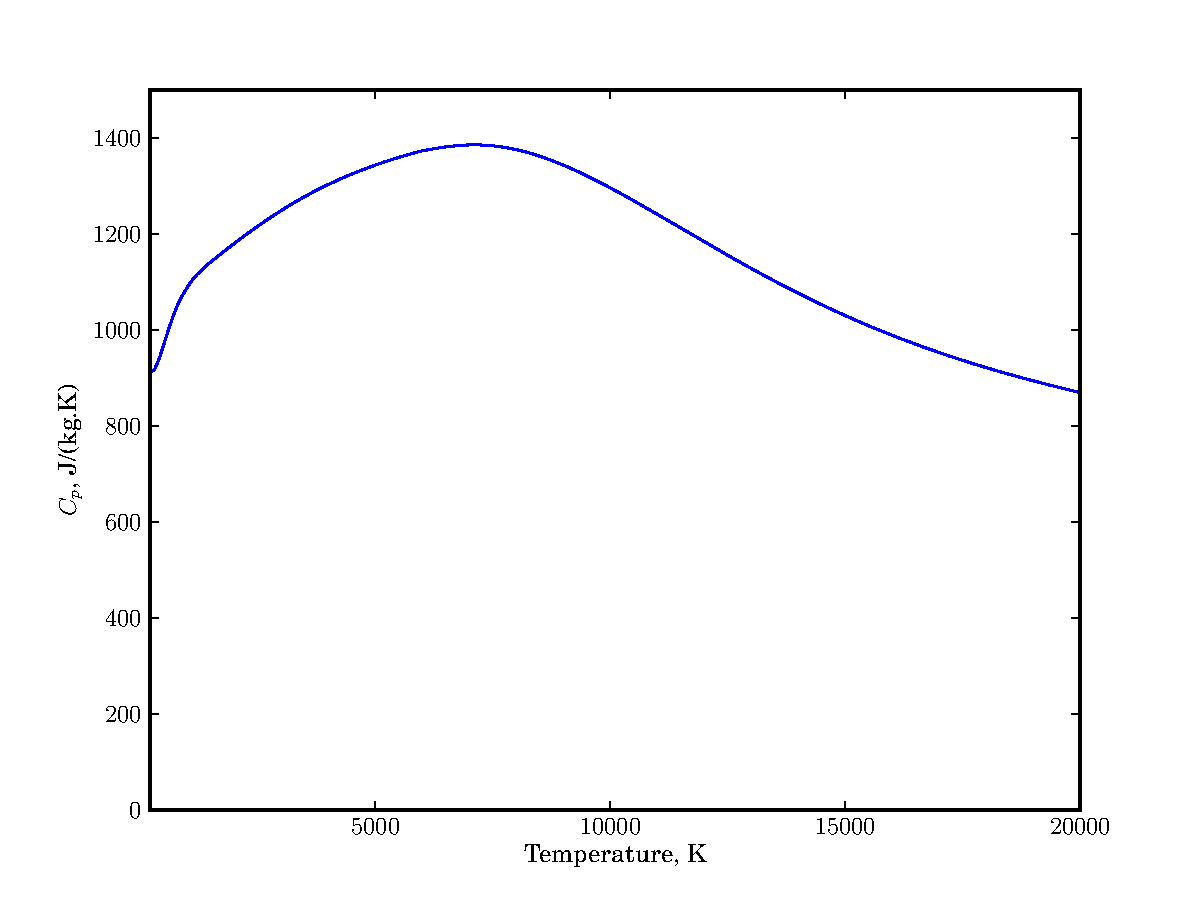
\includegraphics[width=12cm]{../figs/Cp-O2}
\caption[$C_p$ for diatomic oxygen]{Specific heat at constant pressure, $C_p$, for diatomic oxygen as a function of temperature.}
\label{fig:Cp-O2}
\end{figure}

\paragraph{Assumptions}
\begin{itemize}
\item The collisions between particles are perfectly elastic.
\item The particles are point particles; they occupy negligible volume per unit volume.
\item The specific heats $C_p$ and $C_v$ are functions of temperature only.
\end{itemize}
The last assumption implies that the gas is in thermal equilibrium.

\paragraph{Equations}
The \textit{p-v-T} behaviour is simply the perfect gas equation of state:
\begin{equation}
 p = \rho R T \text{ . }
\end{equation}
The internal energy is computed as a function of temperature as
\begin{equation}
 e(T) = \int_{T_0}^{T} C_v(T)\,dT + e_0
\end{equation}
where $e_0$ is the internal energy at a nominated reference state.
For some gases, a function for $C_p$ is available instead of $C_v$.
When that is the case, enthalpy may be evaluated as
\begin{equation}
\label{eq:tpg_h}
 h(T) = \int_{T_0}^{T} C_p(T)\,dT + h_0
\end{equation}
where $h_0$ in the specific enthalpy at a nominated reference state.
The internal energy is then computed from the definition of enthalpy
and applying the perfect gas equation of state:
\begin{equation}
 e = h - RT \text{ . }
\end{equation}

The value of specific entropy can be computed by referencing to
a standard state value $s_0$ at a temperature $T_0$ and pressure
$p_0$:
\begin{equation}
  s(p,T) = \int_{T_0}^{T} \frac{C_p(T)}{T}\,dT - R \log \frac{p}{p_0} + s_0 \text{ . }
\end{equation}

\paragraph{Input parameters}
The input parameters for the thermally perfect gas model
are given in Table~\ref{tab:tpg-params}.
A model for either $C_v$ or $C_p$ as a function
of temperature is required as an input.
Presently, the gas library implementation uses the 
CEA~\cite{mcbride_gordon_1996} polynomials for $C_p$
when modelling a thermally perfect gas.
The details of the CEA polynomials are presented in Appendix~\ref{sec:cea-thermo}.

\begin{table}[h]
\caption{Parameters for the thermally perfect gas model}
\label{tab:tpg-params}
\begin{tabular}{llp{10cm}}
\toprule
Parameter & Units & Description \\ \midrule
\multicolumn{3}{l}{\textit{User input}} \\
$M$       & kg/mole & molecular weight of gas \\
$\gamma$  &  --    & ratio of specific heats, $C_p/C_v$ \\
$T_0$     & K      & temperature at the (user-chosen) standard state \\
$p_0$     & Pa     & pressure at the (user-chosen) standard state \\
$e_0$     & J/kg   & specific internal energy at (user-chosen) standard state.
                    When internal energy is computed, what is really 
                    reported is the \emph{change} in internal energy
                    from this reference or zero-point energy. \\
$s_0$     & J/(kg.K) & specific entropy at the (user-chosen) standard state.
                       As with internal energy, the computed entropy value
                       is the change from the standard state value of entropy. \\
$C_v(T)$ \emph{or} $C_p(T)$ & J/(kg.K) & A model for $C_v$ or $C_p$ as a function of temperature only\\
 & & \\
\multicolumn{3}{l}{\textit{Derived parameter}} \\
$R$      & J/(kg.K) & specific gas constant computed as $R = R_u/M$ where
                      $R_u$ is the universal gas constant \\
\bottomrule
\end{tabular}
\end{table}

\subsection{Real gas}
\paragraph{Description}
At high densities and/or low temperatures, the behaviour of a gas is not well approximated by a perfect gas model.
We model this departure from perfect gas behaviour as a real gas.
The particular form of the \textit{p-v-T} relation varies depending the
model and assumptions that are applied.

\paragraph{Assumptions}
No assumptions about the behaviour of the gas are made.

\paragraph{Equations}
The \textit{p-v-T} relation for a real gas is particular to the
model which is used.
The subsequent sections detail the real gas models available
in the gas library.
In general form, we simply write
\begin{equation}
 p = p(\rho, T) \text{ . }
\end{equation}

The expression for internal energy is written in a general form
by referencing to an energy state, $e_0$, as
\begin{equation}
e = \int_{T_0}^{T} C_v\,dT + \int_{v_0}^{v} \left[ T\left(\frac{\partial p}{\partial T} \right)_v - p \right] dv \text{ . }
\label{eq:int-e-real}
\end{equation}
The evaluation of internal energy is split into two parts.
To compute the first term a model for $C_v$ is required, while the
second term can be computed from a knowledge of the \textit{p-v-T} 
behaviour.

\paragraph{Input parameters}
The ``real gas'' model does not describe any specific gas model,
rather it is generic label.
The specific real gas behaviour is set by selecting a model
for the \textit{p-v-T} behaviour and a model for $C_v$.
Thus Table~\ref{tab:real-gas} just lists the input parameters
in an abstract sense.

\begin{table}[h!]
\caption{Parameters for a real gas model}
\label{tab:real-gas}
\begin{tabular}{llp{10cm}}
\toprule
Parameter & Units & Description \\ \midrule
$M$       & kg/mole & molecular weight of gas \\
\textit{p-v-T} relation & & a model of the \textit{p-v-T} behaviour \\
$C_v$  & J/(kg.K) & a model for $C_v$ \\
\bottomrule
\end{tabular}
\end{table}

\paragraph{Various models of real gas \textit{p-v-T} behaviour}
The following lists the various types of real gases that are modelled
by the gas library.
The details of these models are presented in the subsequent sections.
This list of available real gases is:
\begin{itemize}
\item van der Waal's gas (Section~\ref{sec:van_der_waals_gas})
\item Noble-Abel gas (Section~\ref{sec:noble_abel_gas})
\item Bender gas (Section~\ref{sec:bender_gas})
\end{itemize}

\subsection{van der Waal's gas}
\label{sec:van_der_waals_gas}
\paragraph{Description}
Van der Waal's proposed a modification to the perfect
gas equation of state to account for the intermolecular
forces between particles during collisions and
the finite volume occupied by the particles.

\paragraph{Equations}
The van der Waal's \textit{p-v-T} relation can be written
in terms of density, $\rho$, as
\begin{equation}
  \left ( p + a\rho^2 \right ) \left ( \frac{1}{\rho} - b \right ) = RT \text{ . }
\end{equation}
Substituting this equation in terms of $p$ and $T$ into Equation~\ref{eq:int-e-real} for the internal energy of a real gas, the second term may be integrated to yield an expression for internal energy:
\begin{equation}
e(T, \rho) = \int_{T_0}^{T} C_v\,dT + a \left( \rho - \rho_0 \right) \text{ . }
\end{equation}
Note that this relation still depends on some choice for modelling $C_v$.
Similarly, the second term in the expression for entropy (Eqation~\ref{eq:s-p})
may be evaluated analytically, while the first term depends on the model for $C_v$:
\begin{equation}
s(T,p) = \int_{T_0}^{T} \frac{C_v}{T}\,dT + \left [ R \log \left( v - b \right ) \right ]_{v_0}^{v} \text { . }
\end{equation}


The constants $a$ and $b$ are computed from the critical point pressure and
temperature for the gas.
\begin{equation}
   a = \frac{27 R^2 T^2_{\text{cr}}}{64 P_{\text{cr}}} \qquad \text{and} \qquad
   b = \frac{R T_{\text{cr}}}{8 P_{\text{cr}}}
\end{equation}
Here $b$ is the co-volume of the gas, sometimes written as $\nu_0$.
In the expression above for internal energy, $\rho_0 = \frac{1}{\nu_0}$.

\paragraph{Input parameters}

\begin{table}[h!]
\caption{Parameters for the van der Waal's gas model}
\label{tab:vdw-params}
\begin{tabular}{llp{10cm}}
\toprule
Parameter & Units & Description \\ \midrule
\multicolumn{3}{l}{\textit{User input}} \\
$M$       & kg/mole & molecular weight of gas \\
$T_0$     & K      & temperature at the (user-chosen) standard state \\
$p_0$     & Pa     & pressure at the (user-chosen) standard state \\
$e_0$     & J/kg   & specific internal energy at (user-chosen) standard state.
                    When internal energy is computed, what is really 
                    reported is the \emph{change} in internal energy
                    from this reference or zero-point energy. \\
$s_0$     & J/(kg.K) & specific entropy at the (user-chosen) standard state.
                       As with internal energy, the computed entropy value
                       is the change from the standard state value of entropy. \\
$p_c$     & Pa     & critical point pressure \\
$T_c$     & K      & critical point temperature \\
 & & \\
\multicolumn{3}{l}{\textit{Derived parameters}} \\
$R$      & J/(kg.K) & specific gas constant computed as $R = R_u/M$ where
                      $R_u$ is the universal gas constant \\
$a$      & J$^2$/(kg$^2$Pa) & constant accounting for the effect of intermolecular forces
                              computed as \[ a = \frac{27 R^2 T^2_{\text{cr}}}{64 P_{\text{cr}}} \] \\
$b$      & m$^3$/kg & co-volume (sometimes seen as $\nu_0$) computed as
                      \[ b = \frac{R T_{\text{cr}}}{8 P_{\text{cr}}} \] \\

\bottomrule
\end{tabular}
\end{table}

\subsection{Noble-Abel gas}
\label{sec:noble_abel_gas}
\paragraph{Description}
The Noble-Abel gas model for real gas behaviour is a simplication of
the van der Waal's model in that it only accounts for the co-volume
occupied by the gas particles.
This model is applicable at high pressures where the volume of
the particles is an appreciable fraction of the total occupied volume
but the collision interactions are not significantly affected
by intermolecular forces.
This may be the case at high temperatures where the collisions
occur relatively quickly, not allowing much time for the intermolecular
forces to exert an effect.
The Noble-Abel gas model is frequently used when simulating interior
ballistics.

\paragraph{Equations}
The \textit{p-v-T} behaviour for a Noble-Abel gas is expressed as
\begin{equation}
  p \left( \frac{1}{\rho} - b \right ) = RT \text{ . }
\end{equation}

Since $\left( \frac{\partial p}{\partial T} \right)_v$ evaluates to the same analytical expression as in the case of a van der Waal's case, the expressions for internal
energy and entropy are the same:
\begin{equation}
e(T, \rho) = \int_{T_0}^{T} C_v\,dT + a \left( \rho - \rho_0 \right) \text{ , }
\end{equation}
and 
\begin{equation}
s(T,p) = \int_{T_0}^{T} \frac{C_v}{T}\,dT + \left [ R \log \left( v - b \right ) \right ]_{v_0}^{v} \text { . }
\end{equation}

Again, the co-volume $b$ is computed as
\begin{equation}
   b = \frac{R T_{\text{cr}}}{8 P_{\text{cr}}} \text{ . }
\end{equation}
Note, sometimes $b$ is specified directly for certain gases.
It may be more accurate to use an empirically-derived value
over a certain pressure and temperature range.

\paragraph{Input parameters}

\begin{table}[h]
\caption{Parameters for the Noble-Abel gas model}
\label{tab:na-params}
\begin{tabular}{llp{10cm}}
\toprule
Parameter & Units & Description \\ \midrule
\multicolumn{3}{l}{\textit{User input}} \\
$M$       & kg/mole & molecular weight of gas \\
$T_0$     & K      & temperature at the (user-chosen) standard state \\
$p_0$     & Pa     & pressure at the (user-chosen) standard state \\
$e_0$     & J/kg   & specific internal energy at (user-chosen) standard state.
                    When internal energy is computed, what is really 
                    reported is the \emph{change} in internal energy
                    from this reference or zero-point energy. \\
$s_0$     & J/(kg.K) & specific entropy at the (user-chosen) standard state.
                       As with internal energy, the computed entropy value
                       is the change from the standard state value of entropy. \\
$p_c$     & Pa     & critical point pressure \\
$T_c$     & K      & critical point temperature \\
 & & \\
\multicolumn{3}{l}{\textit{Derived parameters}} \\
$R$      & J/(kg.K) & specific gas constant computed as $R = R_u/M$ where
                      $R_u$ is the universal gas constant \\
$b$      & m$^3$/kg & co-volume (sometimes seen as $\nu_0$) computed as
                      \[ b = \frac{R T_{\text{cr}}}{8 P_{\text{cr}}} \] \\

\bottomrule
\end{tabular}
\end{table}

\subsection{Bender gas}
\label{sec:bender_gas}

\paragraph{Description}
\paragraph{Assumptions}
\paragraph{Equations}
\paragraph{Input parameters}


\subsection{Perfect gas mixtures}
\label{sec:pgm}
\paragraph{Description}
A perfect gas mixture, as the name implies, is a gas composed
of individual components each having perfect gas behvaiour.
This model is typically used when simulating chemically
reacting gases; each chemical species is treated as a separate
component of the gas mixture.
Usually, it makes physical sense to assume that each of the component species
has the same thermal behaviour.
This leads to the special cases of calorically perfect gas mixtures and
thermally perfect gas mixtures.
The equations describing the mixture properties are the same in both
instances. 

\paragraph{Assumptions}
\begin{itemize}
\item Each component of the gas exhibits perfect behaviour.
\item The Gibbs-Dalton law holds: the properties of individual
      component gases are not influenced by the presence of
      other gases, and each component in the mixture behaves
      as if it existed alone at mixture temperature and volume.
\end{itemize}

\paragraph{Equations}
For mixtures, the thermodynamic state is uniquely defined
by specifying two independemt properties of the mixture and the mixture
composition.
The subscript $m$ is used to denote mixture properties.
By applying Dalton's Law of partial pressures, the
\textit{p-v-T} behaviour for a mixture of perfect
gases is
\begin{equation}
 p_m = \sum_{i=1}^N \rho_i R_i T \text{ . }
\end{equation}
The internal energy for the mixture, $e_m$, is computed as
a mass fraction weighted sum of the component
internal energies
\begin{equation}
 e_m = \sum_{i=1}^N f_i e_i(T_m) \text{ . }
\end{equation}
A number of other mixture properties are also computed
as a mass fraction weighted sum.
The entropy of the mixture is
\begin{equation}
 s_m = \sum_{i=1}^N f_i s_i(T_m, p_m) \text{ . }
\end{equation}
The specific gas constant of the mixture is
\begin{equation}
 R_m = \sum_{i=1}^N f_i R_i \text{ . }
\end{equation}
The specific heats are
\begin{equation}
  C_{p_m} = \sum_{i=1}^N f_i C_{p_i} \text{ , }
\end{equation}
and
\begin{equation}
  C_{v_m} = \sum_{i=1}^N f_i C_{v_i} \text{ . }
\end{equation}
The mixture molecular weight is computed as a mole fraction
weighted sum as
\begin{equation}
  M_m = \sum_{i=1}^N y_i M_i \text{ . }
\end{equation}

\paragraph{Input parameters}
The input for the model is a list of the component gaseous species.
For each species, a specific perfect gas model needs to be selected
(and appropriate inputs given).
The available gas models for the componets is a selection of a calorically perfect
gas (Section~\ref{sec:cal-perf}) or thermally perfect gas (Section~\ref{sec:therm-perf}).

\subsection{Real gas mixtures}
\paragraph{Description}
The model of real gas mixtures assumes that all of the
component gases have real gas behaviour.
This model is useful for interior ballistics simulations
where there are a number of component gases such
as air and propellant combustion products.

\paragraph{Assumptions}
The properties for a mixture of real gases are more complex to compute
than those for a mixture of real gases.
Dalton's Law of Partial Pressures and Amagat's Law of Additive Volumes
do not hold exactly but can be applied to give an approximate
treatment.
An alternative approach, and the one used in the gas library,
is to assume the gas mixture behaves as a pseudopure substance.

\paragraph{Equations}
The \textit{p-v-T} behaviour of the gas is computed by assuming
either van der Waal's behaviour
\begin{equation}
  \left ( p_m + a_m\rho_m^2 \right ) \left ( \frac{1}{\rho_m} - b_m \right ) = R_mT_m \text{ , }
\end{equation}
or Noble-Abel behaviour
\begin{equation}
  p_m \left( \frac{1}{\rho_m} - b_m \right ) = R_mT_m \text{ . }
\end{equation}
The mixture constants $a_m$ and $b_m$ are computed as
\begin{equation}
  a_m = \left( \sum_{i=1}^N y_i \sqrt{a_i} \right)^2 \qquad \text{and} \qquad 
  b_m = \sum_{i=1}^N y_i b_i \text{ . }
\end{equation}
The mixture gas constant is as 
\begin{equation}
R_m = \sum_{i=1}^N f_i R_i \text{ . }
\end{equation}
The remainder of the mixture properties are computed in
the same manner as for the mixture of perfect gases (see Section~\ref{sec:pgm}).


\paragraph{Input parameters}
The input for the model is a list of the component gaseous species and
the type of real gas model (either van der Waal's or Noble-Abel).
For each species, the parameters for the specific real gas model need to be set.

\subsection{Multi-temperature gas mixtures}
\label{sec:multi-T}
\paragraph{Description}
\paragraph{Assumptions}
\paragraph{Equations}
\paragraph{Input parameters}



\chapter{Transport Properties}
\label{chap:trans-prop}

\chapter{Chemical Kinetics}
\label{chap:chem-kinetics}

Chemical nonequilibrium flows, also called flows with finite-rate chemical effects,
are an important class of flows in the study of gas dynamics.
On a kinetic level, chemical nonequilibrium exists in the gas when there have not been 
sufficient particle collisions to reach chemical equilibrium
at a given pressure and temperature.
In terms of modelling fluid dynamics, the influence of chemical nonequilibrium
effects is important when the time for completion of the chemical reactions
is of the same order of magnitude as some characteristic flow time scale.
Consider
$\tau_f$ as a characteristic transit time for the flow and $\tau_c$ as a characteristic chemical relaxation time; this leads to a convenient classification of types of flows:
\begin{description}
  \item[frozen flow] the time taken for chemical relaxation is much longer
                     than the flow transit time of interest
                     \[ \tau_c \gg \tau_f \]
  \item[nonequilibrium flow] the time taken for chemical relaxation is comparable
                             to the time for flow transit (and influential on that flow)
                             \[ \tau_c \approx \tau_f \]
  \item[equilibrium flow] the time taken for chemical relaxation time is much quicker
                          than the flow transit time
                          \[ \tau_c \ll \tau_f \]
\end{description}

In gas dynamics, the influence of chemical nonequilibrium processes
is important in a number of classes of flow such as:
\begin{itemize}
\item blunt body flows during planetary-entry;
\item combustion processes;
\item detonation waves; and
\item nozzle flows.
\end{itemize}
The same basic theoretical treatment
can be applied to each of theses types of flows.
In this section, the model for computing 
the gas phase chemical reactions in nonequilibrium flows is described.


\section{Rates of species change}
\label{subsec:chem_rates}
By assuming a set of simple reversible reactions,
the chemically reacting system can be represented as,
\begin{equation}
   \sum_{i=1}^N \alpha_i X_i \rightleftharpoons \sum_{i=1}^N \beta_i X_i,
\end{equation}
where $\alpha_i$ and $\beta_i$ represent the stoichiometric coefficients for the reactants and
products respectively, and $X_i$ is the concentration of species $i$.
The case of an irreversible reaction is represented by setting the backward rate to zero.
For a given reaction $j$, the rate of concentration change of species $i$ is given as,
\begin{equation}
  \left( \frac{d[X_i]}{dt} \right)_j = \nu_i \left\{ k_f \prod_i [X_i]^{\alpha_i} 
                       - k_b \prod_i [X_i]^{\beta_i} \right\},
\end{equation}
where $\nu_i = \beta_i - \alpha_i$.
By summation over all reactions, $N_r$, the total rate of concentration change is,
\begin{equation}
\label{eqn:chem_ode_system}
  \frac{d[X_i]}{dt} = \sum_{j=1}^{N_r} \left( \frac{d[X_i]}{dt} \right)_j.
\end{equation}
For certain integration schemes it is convenient to have the production and loss
rates available as separate quantities.
In this case,
\begin{equation}
\label{eq:split}
  \frac{d[X_i]}{dt} = q_i - L_i = \sum_{j=1}^{N_r} \dot{\omega}_{app_{i,j}} - \sum_{j=1}^{N_r} \dot{\omega}_{va_{i,j}} 
\end{equation}
The calculation of $\dot{\omega}_{app_{i,j}}$ and $\dot{\omega}_{va_{i,j}}$ depends on the
value of $\nu_i$ in reach reaction $j$ as shown in Table~\ref{tab:omega}.

\begin{table}[h]
\caption[Chemical production and loss terms]{The form of the chemical production and loss terms based on the value of $\nu_i$}
\label{tab:omega}
\begin{center}
\begin{tabular}{ccc}
\hline \hline
                           & $\nu_i > 0$                          & $\nu_i < 0$  \\ \hline
 $\dot{\omega}_{app_{i}}$  & $\nu_i k_f \prod_i [X_i]^{\alpha_i}$ & $-\nu_i k_b \prod_i [X_i]^{\beta_i}$ \\
 $\dot{\omega}_{va_{i}}$   & $-\nu_i k_b \prod_i [X_i]^{\beta_i}$ & $\nu_i k_f \prod_i [X_i]^{\alpha_i}$ \\ \hline \hline
\end{tabular}
\end{center}
\end{table}

The calculation of the reaction rate coefficients, $k_f$ and $k_b$, is described in
Section~\ref{sec:reac_coeffs} and the solution methods for the ordinary differential
equation system of species concentration changes is presented in Section~\ref{sec:ODE}.

\section{Reaction rate coefficients}
\label{sec:reac_coeffs}

The reaction rate coefficients for a reaction can be determined by experiment (often
shock tube studies are used) or from theory.
In a great number of cases, estimates of the reaction rate from theory can vary by
orders of magnitude from experimentally determined values.
For this reason, fits to experimental values are most commonly used.
The methods for computing reaction rate coefficients available in the
gas library are described below.

\paragraph{A note on the units of reaction rate coefficients}



\subsection{Generalised Arrhenius rate coefficients}
\paragraph{Description}
The Arrhenius rate form is used to approximate reaction
rates derived from either experimental data
or theoretical calculations.

\paragraph{Equations}

The generalised Arrhenius expression for a rate coefficient, either forwards or backwards, is
\begin{equation}
\label{eqn:ga}
k = A T^{n} \exp{\left( \frac{-E_a}{k_bT}\right)}
\end{equation}
where $k_b$ is the Boltzmann constant and $A$, $n$ and $E_a$ are constants
of the model.
This may be written equivalently in terms of an activation
temperature, $T_a = E_a/k_b$, as
\begin{equation}
k = A T^{n} \exp{\left( \frac{-T_a}{T}\right)} \text{ . }
\end{equation}


The original Arrhenius formula does not include the pre-exponentiation
temperature cofactor, $T^n$.
In the gas library, the simpler Arrhenius formula is not
a separate modelling option.
Instead, one sets $n = 0$, to get
\begin{equation}
k = A \exp{\left( \frac{-E_a}{k_bT}\right)} \text{ . }
\end{equation}

\paragraph{Input parameters}

\begin{table}[h!]
\caption{Parameters for the generalised Arrhenius rate formula}
\label{tab:ga-formula}
\begin{tabular}{llp{10cm}}
\toprule
Parameter & Units & Description \\ \midrule
\multicolumn{3}{l}{\textit{User input}} \\
$A$       & ${}^*$ & pre-exponential coefficient in c.g.s units.
                    ${}^*$ The units vary depending on the particular
                    elementary reaction. For example, for bimolecular reactions,
                    the units of $A$ are cm$^3$/(mole.s). \\
$n$       &  --    & the power of the pre-exponentiation temperature cofactor \\
$T_a$     & K      & activation temperature \\
\bottomrule
\end{tabular}
\end{table}
When the reaction rate coefficient is given in terms
of activation energy, $E_a$, the equivalent activation
temperature is calculate as
\[ T_a = \frac{E_a}{k_b} \text{ . } \]


\subsection{Using the equilibrium constant to compute rate coefficients}
\paragraph{Description}
The Law of Mass Action can be used to relate the forwards
and backwards rate coefficient from the equilibrium constant.
This is useful when the reaction rate coefficient
is only given for one direction of the reaction.

\paragraph{Equations}
Given either a forwards or backwards rate coefficient, the
other coefficient may be obtained from the expression
\begin{equation}
K_c = \frac{k_f}{k_b}
\end{equation}
where $K_c$ is the equilibrium constant calculated based
on concentrations.

The equilibrium constant is sometimes computed from curve fits
or can be computed from thermodynamics principles.
In the gas library implementation, the equilibrium constant
is computed from first principles.
The equilibrium constant based on concentration is related to the equilibrium constant
based on pressure by,
\begin{equation}
K_c = K_p \left( \frac{p_{atm}}{R_uT} \right)^{\nu}
\end{equation}
where $p_{atm}$ is atmospheric pressure in Pascals, $R_u$ is the universal
gas constant, and $\nu = \sum_i^{N_S} \nu_i$.
The equilibrium constant based on pressure is
\begin{equation}
K_p = \exp{\left( \frac{-\Delta G^*(T)}{R_uT} \right) }.
\end{equation}
The derivation of the formula for $K_p$,
the equilibrium constant based on partial pressures,
can be found in any introductory text on classical thermodynamics
which covers chemical equilibrium.
The standard state differential Gibbs function for the reaction,
$\Delta G^*(T)$, is defined as
\begin{equation}
\Delta G^*(T) = \sum_i^{N_s} \nu_i \bar{g}_i^*(T)
\end{equation}
where each $\bar{g}_i^*$ is the molal Gibbs free energy 
at a pressure of one atmosphere,
\begin{equation}
\bar{g}_i^*(T) = \bar{h}_i(T) - T \bar{s}_i(T) \text{ . }
\end{equation}

\paragraph{Input parameters}
No input parameters are required.
The necessary inputs are part of the thermodynamics
model input.

\subsection{Pressure-dependent rate coefficients}

BRENDAN TO ADD CONTENT.



\chapter{Energy Exchange Kinetics}
\label{chap:ee-kinetics}






\part{User's Guide}
\chapter{Installation}
\label{chap:install}

The core of the radiation module is written in C++, and there are a number of tools written in Python.
The input data is provided to the C++ binaries via Lua files.
Assuming the Compressible-Flow CFD repository is located in \verb ~/cfcfd3-hg , the radiation module can be compiled and installed via:

\begin{lstlisting}[basicstyle=\ttfamily\small]
$ cd ~/cfcfd3-hg/lib/radiation/build
$ make install
\end{lstlisting}

The installation of the radiation library can then be tested via an automated script:

\begin{lstlisting}[basicstyle=\ttfamily\small]
$ cd ~/cfcfd3-hg/lib/radiation/build
$ make test
\end{lstlisting}

If the user has the SPRADIAN07 code available and wishes to use it as the spectral model, this needs to be requested at compile time:

\begin{lstlisting}[basicstyle=\ttfamily\small]
$ cd ~/cfcfd3-hg/lib/radiation/build
$ make WITH_SPRADIAN=1 install
\end{lstlisting}

The SPRADIAN07 source code and input-data files need to be located in \\
\verb ~/cfcfd3-hg/extern/spradian07 :

\begin{lstlisting}[basicstyle=\ttfamily\small]
$ ls ~/cfcfd3-hg/extern/spradian07/
atom.dat     diatom.dat   radipac6.f90 triatom.dat
\end{lstlisting}

If the Parade code is availale to the user, no additional compilation arguments are need 
to use it as the spectral model.
The \texttt{parade} binary, however, needs to be in the system path and the Parade template file needs to include the location of the Parade data files (the Parade template file can be automatically generated from the python input script - see \texttt{lib/radiation/test/parade-air-EQ-radiators.py} for an example).

\par

To test all the spectral models the following make command can be run:

\begin{lstlisting}[basicstyle=\ttfamily\small]
$ cd ~/cfcfd3-hg/lib/radiation/build
$ make WITH_SPRADIAN=1 WITH_PARADE=1 test
\end{lstlisting}

\chapter{Getting Started}

\chapter{Creating Input Files}
\label{chap:input}

The input data to create a new spectral radiation model is provided in a Lua file.
This file contains all the parameters and spectroscopic data to perform a spectral radiation calculation.
To simplify the creation of this file for the user, the Lua file can be created via the \texttt{script\_rad2.py} Python tool that interfaces with a library of spectroscopic data.
Instructions on how to use this tool can be obtained from the command line via:

\begin{lstlisting}[basicstyle=\ttfamily\small]
$ script_rad2.py --help
Usage: script_rad2.py -i rad_desc.py|--input-script=rad_desc.py
                      -L LUA_output.lua|--LUA-file=LUA_output.lua

Options:
  -h, --help            show this help message and exit
  -i INFILE, --input-script=INFILE
                        input Python script for radiation description
  -L LUAFILE, --LUA-file=LUAFILE
                        output configuration file for 'librad2' C++ module in
                        LUA format
\end{lstlisting}

\noindent where \texttt{rad-model.py} is the name of the user created Python script describing the spectral model and \texttt{rad-model.lua} is the desired name of the resulting Lua file.
A sample user-created Python script for creating a basic radiation model for 11 species, 2 temperature air is shown below:

\noindent \topbar
\lstinputlisting[language=python,caption={Example spectral model input file, \texttt{air-radiators.py}}]{../../../testing/air-radiators.py}
\bottombar

In `\texttt{1.}', the desired spectral model is selected:

\begin{lstlisting}[basicstyle=\ttfamily\small]
# 1. Select the spectral model
gdata.spectral_model = "photaura"
\end{lstlisting}

Here the in-house \texttt{photaura} model has been selected; other available models are \texttt{spradian} and \texttt{parade}.
See Appendix~\ref{} for an example of how to construct an input file for these.
The spectral grid is then defined in '\texttt{2.}':

\begin{lstlisting}[basicstyle=\ttfamily\small]
# 2. Define the spectral grid
gdata.lambda_min = 50.0
gdata.lambda_max = 1000.0
gdata.spectral_points = 95000
\end{lstlisting}

\noindent Here the range $50 \leq \lambda \leq 1000$~nm has been requested, discretised by 95000 equidistant points in frequency space.
Presently only spectral domains with consant frequency intervals are permitted.
Finally, in '\texttt{3.}' the desired radiating species are requested and defined:

\begin{lstlisting}[basicstyle=\ttfamily\small]
# 3. Request and define the radiating species
species   = [ "N2", "N2_plus", "NO", "NO_plus", "O2", "O2_plus",
               "N",  "N_plus",  "O",  "O_plus", "e_minus" ]
radiators = [ "N2", "N2_plus", "NO", "O2", "N", "N_plus",
              "O", "O_plus", "e_minus" ]
for rad_name in radiators:
    rad = gdata.request_radiator(rad_name)
    rad.default_data()
    rad.isp = species.index(rad_name)
    rad.iTe = 1
    if rad.type == "diatomic_radiator":
        rad.iTv = 1
\end{lstlisting}

A radiator is requested from the library with the \texttt{gdata.request\_radiator()} function call.
If the radiator is not present in the library, \texttt{script\_rad2.py} will fail here with an error message indicating what species was not avaiable.  
The \texttt{rad.default\_data()} function requests the nominal electronic level and transition probability set from the library -- for most calculations this will be suitable.
Other data that is set here is the species index in the \texttt{rad.isp} field, the electronic temperature index in the \texttt{rad.iTe} field and the vibrational temperature index in the \texttt{rad.iTv} field.  
\chapter{Use in CFD Code}
\label{chap:cfd}

\chapter{Use of the Python Module}
\label{chap:python}

\chapter{Examples}
\label{chap:examples}



\part{Developer's Guide}
\include{code-organisation}
\include{lua-input}
\include{dsls}

\renewcommand\bibname{References}
\bibliographystyle{unsrt}
\bibliography{gas,equations-of-state}
\addcontentsline{toc}{chapter}{References}

\appendix
\addcontentsline{toc}{part}{Appendix}
\chapter{Application Programming Interface}
\label{app:api}

\chapter{Look-up Table Format}
\label{app:lut}

\chapter{User-defined gas model}

\chapter{Polynomials and curve fits for property evaluations}
\label{chap:poly}

\section{CEA polynomials for thermodynamic properties}
\label{sec:cea-thermo}
The CEA polynomials can be used to evaluate the specific heat
at constant pressure ($C_p$), enthalpy ($h$), and
the temperature-dependent component of entropy ($s^o$).
For a given species, the polynomials are split over various temperature
ranges of validity.
Typically, the coefficients for the polynomials are valid over temperature ranges
from 200.0 -- 1000.0\,K and and 1000.0 -- 6000.0\,K.
For some species, there is a high-temperature range from 6000.0 -- 20,000.0\,K.
The CEA thermodynamics database gives are nine coefficients ($a_0 \ldots a_8$) for each polynomial piece.
Additionally, an enthalpy of formation is listed for each species.
This may be used as the reference enthalpy value in Equation~\ref{eq:tpg_h}.
The polynomials in non-dimensional form are:
\begin{eqnarray}
 \frac{C_p(T)}{R} & = & a_0 T^{-2} + a_1 T^{-1} + a_2 + a_3 T + a_4 T^2 + a_5 T^3 + a_6 T^4 \\
 \frac{h(T)}{RT} & = & -a_0 T^{-2} + a_1 T^{-1} \log{T} + a_2 + a_3 \frac{T}{2} +
                        a_4 \frac{T^2}{3} + a_5 \frac{T^3}{4} + a_6 \frac{T^4}{5} + \frac{a_7}{T} \\
 \frac{s^o(T)}{R} & = & -a_0 \frac{T^{-2}}{2} - a_1 T^{-1} + a_2 \log{T} + a_3 T + a_4 \frac{T^2}{2}  +
                        a_5 \frac{T^{3}}{3} + a_6 \frac{T^4}{4} + a_8
\end{eqnarray}

\section{CEA polynomials for transport properties}
\begin{equation}
\log{\mu(T)}  =  a_0 \log{T} + \frac{a_1}{T} + \frac{a_2}{T^2} + a_3
\end{equation}
\begin{equation}
\log{k(T)} = b_0 \log{T} + \frac{b_1}{T} + \frac{b_2}{T^2} + b_3
\end{equation}


% code.tex

\newpage
\section{Code}
\label{code}

The following is the space marching solver code extracted directly out of the \textit{main.cxx} file from eilmer3.

{\scriptsize
\begin{verbatim}
int integrate_blocks_in_sequence( void )
// This procedure integrates the blocks one-at-a-time in sequence.
//
// The idea is to approximate the space-marching approach of sm_3d
// and, hopefully, achieve a significant speed-up over integration
// of the full array of blocks.
//
// It is assumed that we have the restricted case 
// of all the blocks making a single line (west to east) with
// supersonic flow at the west face of block 0 and 
// extrapolate_out on the east face of the final block.
//
// The above assumptions still stand but the code has been modified
// such that the calcluation now does two active blocks at a time.
// The calculation initially does blocks 0 and 1, and then moves over
// one block for the next step calculating blocks 1 and 2 next.
// This process is then repeated for the full calculation

{
    global_data &G = *get_global_data_ptr();
    Block *bdp;
    double time_slice = G.max_time / G.nblock;
    BoundaryCondition *bcp_save;

    // Initially deactivate all blocks
    for ( int jb = 0; jb < G.nblock; ++jb ) {
	bdp = get_block_data_ptr(jb);
	bdp->active = 0;
    }

    cout << "Integrate Block 0 and Block 1" << endl;

    // Start by setting up block 0

    // Activate block 0
    bdp = get_block_data_ptr(0);
    bdp->active = 1;
    // Apply the assumed SupINBC to the west face and propogate across the block
    bdp->bcp[WEST]->apply_inviscid(0.0);
    bdp->propagate_data_west_to_east( G.dimensions );
    bdp->apply( &FV_Cell::encode_conserved, bdp->omegaz, "encode_conserved" );
    // Even though the following call appears redundant at this point,
    // fills in some gas properties such as Prandtl number that is
    // needed for both the cfd_check and the BLomax turbulence model.
    bdp->apply( &FV_Cell::decode_conserved, bdp->omegaz, "decode_conserved" );

    // Now set up block 1

    // Activate block 1
    bdp = get_block_data_ptr(1);
    bdp->active = 1;

    // Save the original east boundary condition and apply the temporary
    // ExtrapolateOutBC for the calculation
    bcp_save = bdp->bcp[EAST];
    bdp->bcp[EAST] = new ExtrapolateOutBC(*bdp, EAST, 0);

    // Read in data from block 0 and propogate across the block
    exchange_shared_boundary_data( 1, COPY_FLOW_STATE);
    bdp->propagate_data_west_to_east( G.dimensions );
    bdp->apply( &FV_Cell::encode_conserved, bdp->omegaz, "encode_conserved" );
    bdp->apply( &FV_Cell::decode_conserved, bdp->omegaz, "decode_conserved" );

    // Integrate just the first two blocks in time, hopefully to steady state.
    set_block_range(0,1);
    integrate_in_time( time_slice );


    // The rest of the blocks.
    for ( int jb = 2; jb < (G.nblock); ++jb ) {
	// jb-2, jb-1, jb
	// jb-2 is the block to be deactivated, jb-1 has been iterated and now
	// becomes the left most block and jb is the new block to be iterated
	cout << "Integrate Block " << jb << endl;
	// Make the block jb-2 inactive.
	bdp = get_block_data_ptr(jb-2);
	bdp->active = 0;

	// block jb-1 - reinstate the previous boundary condition on east face
	// but leave the block active
	bdp = get_block_data_ptr(jb-1);
	delete bdp->bcp[EAST];
	bdp->bcp[EAST] = bcp_save;

	// Set up new block jb to be integrated
	bdp = get_block_data_ptr(jb);
	bdp->active = 1;

	if ( jb < G.nblock-1 ) {
	    // Cut off the east boundary of the current block 
	    // from the downstream blocks if there are any.
	    bcp_save = bdp->bcp[EAST];
	    bdp->bcp[EAST] = new ExtrapolateOutBC(*bdp, EAST, 0);
	}
	// Now copy the starting data into the WEST ghost cells
	// and propagate it across the current block.
	exchange_shared_boundary_data( jb, COPY_FLOW_STATE );
	bdp->propagate_data_west_to_east( G.dimensions );
	bdp->apply( &FV_Cell::encode_conserved, bdp->omegaz, "encode_conserved" );
	bdp->apply( &FV_Cell::decode_conserved, bdp->omegaz, "decode_conserved" );
	// Integrate just the two currently active blocks in time,
	// hopefully to steady state.
	set_block_range(jb-1, jb);
	integrate_in_time( (jb+1)*time_slice );
    }
    // Before leaving, we want all blocks active for output.
    for ( int jb = 0; jb < G.nblock; ++jb ) {
	bdp = get_block_data_ptr(jb);
	bdp->active = 1;
    }
    set_block_range(0, G.nblock - 1);
    return SUCCESS;
} // end integrate_blocks_in_sequence()
}
\end{verbatim}
}

\end{document}
